\documentclass[11pt,a4paper]{article}
\usepackage[utf8]{inputenc}
\usepackage[text={17cm, 24cm}, left=2cm, top=3cm]{geometry}
\usepackage[czech]{babel}
\usepackage{times}
\usepackage{url}
\urlstyle{rm}
\usepackage{multirow}
\usepackage{algorithm}
\usepackage{algpseudocode}
\usepackage{graphics}
\usepackage{pdflscape}

\begin{document}
\begin{titlepage}
    \begin{center}
        \textsc{\Huge Vysoké učení technické v Brně             
        \bigskip \\}
        \textsc{\huge Fakulta informačních technologií}
        \vspace{\stretch{0.382}}
        
        {\LARGE Typografie a publikování - 3. projekt \\
            \vspace{0.3em}
        \Huge Tabulky a obrázky}
        \vspace{\stretch{0.618}}
        
        {\Large \today \hfill 
        Zdeněk Dobeš}
    \end{center}
\end{titlepage}

\section{Úvodní strana}
Název práce umístěte do zlatého řezu a nezapomeňte uvést \uv{dnešní} datum a vaše jméno a příjmení.

\section{Tabulky}

Pro sázení tabulek můžeme použít buď prostředí \ \texttt{tabbing} \ nebo prostředí \ \texttt{tabular.}

\subsection{Prostředí \ \texttt{tabbing}}

Při použití \ \texttt{tabbing} \ vypadá tabulka následovně:

\begin{tabbing}
Vodní melouny \quad \= 25,90 \quad \= 2,5 kg \= \kill
\textbf{Ovoce} \> \textbf{Cena} \> \textbf{Množství} \\
Jablka \> 25,90 \> 3 kg \\
Hrušky \> 27,40 \> 2,5 kg \\
Vodní melouny \> 35,- \> 1 kus \\
\end{tabbing}
Toto prostředí se dá také použít pro sázení algoritmů, ovšem vhodnější je použít prostředí \texttt{algorithm} nebo \linebreak \texttt{algorithm2e} (viz sekce \ref{Algoritmy}).

\subsection{Prostředí \texttt{tabular}}

Další možností, jak vytvořit tabulku, je použít prostředí \texttt{tabular.} Tabulky pak budou vypadat takto\footnote{Kdyby byl problém s \texttt{cline}, zkuste se podívat třeba sem: \normalfont \url{http://www.abclinuxu.cz/tex/poradna/show/325037}.}: \\
\begin{table}[h]
\begin{center}
\catcode`\-=12
    \begin{tabular}{|c|c|c|}
    \hline
     & \multicolumn{2}{c}{\textbf{Cena}} \vline \\ \cline{2-3}
   \textbf{Měna} & \textbf{nákup} & \textbf{prodej} \\ \hline
    EUR & 24,775 & 25,943 \\
    GBP & 29,394 & 30,492 \\
    USD & 22,423 & 23,661 \\ \hline
    \end{tabular}
    \caption{Tabulka kurzů k dnešnímu dni}
    \label{tab_1}
\end{center}
\end{table}

\begin{table}[h]
\begin{center}
\begin{tabular}{|c|c|}
\hline
$A$ & $\neg$ A \\ \hline
\textbf{P} & N \\ \hline
\textbf{O} & O \\ \hline
\textbf{X} & X \\ \hline
\textbf{N} & P \\
\hline
\end{tabular}
\vspace{1mm}
\catcode`\-=12
\begin{tabular}{|c|c|c|c|c|c|}
\hline
\multicolumn{2}{|c}{\multirow{2}{*}{$A \wedge B$}} \vline & \multicolumn{4}{c}{$B$} \vline \\
\cline{3-6}
\multicolumn{2}{|c}{} \vline & \textbf{P} & \textbf{O} & \textbf{X} & \textbf{N} \\ \hline
\multirow{4}{*}{$A$} & \textbf{P} & P & O & X & N \\ \cline{2-6}
\multirow{4}{*}{} & \textbf{O} & O & O & N & N \\ \cline{2-6}
\multirow{4}{*}{} & \textbf{X} & X & N & X & N \\ \cline{2-6}
\multirow{4}{*}{} & \textbf{N} & N & N & N & N \\ \hline
\end{tabular}
\vspace{1mm}
\begin{tabular}{|c|c|c|c|c|c|}
\hline
\multicolumn{2}{|c}{\multirow{2}{*}{$A \vee B$}} \vline & \multicolumn{4}{c}{$B$} \vline \\
\cline{3-6}
\multicolumn{2}{|c}{} \vline & \textbf{P} & \textbf{O} & \textbf{X} & \textbf{N} \\ \hline
\multirow{4}{*}{$A$} & \textbf{P} & P & P & P & P \\ \cline{2-6}
\multirow{4}{*}{} & \textbf{O} & P & O & P & O \\ \cline{2-6}
\multirow{4}{*}{} & \textbf{X} & P & P & X & X \\ \cline{2-6}
\multirow{4}{*}{} & \textbf{N} & P & O & X & N \\ \hline
\end{tabular}
\vspace{1mm}
\begin{tabular}{|c|c|c|c|c|c|}
\hline
\multicolumn{2}{|c}{\multirow{2}{*}{$A \rightarrow B$}} \vline & \multicolumn{4}{c}{$B$} \vline \\
\cline{3-6}
\multicolumn{2}{|c}{} \vline & \textbf{P} & \textbf{O} & \textbf{X} & \textbf{N} \\ \hline
\multirow{4}{*}{$A$} & \textbf{P} & P & O & X & N \\ \cline{2-6}
\multirow{4}{*}{} & \textbf{O} & P & O & P & O \\ \cline{2-6}
\multirow{4}{*}{} & \textbf{X} & P & P & X & X \\ \cline{2-6}
\multirow{4}{*}{} & \textbf{N} & P & P & P & P \\ \hline
\end{tabular}
\caption{Protože Kleeneho trojhodnotová logika už je \uv{zastaralá}, uvádíme si zde příklad čtyřhodnotové \\\hspace{1cm} logiky}
\label{tab_2}
\end{center}
\end{table}

\pagebreak

\section{Algoritmy}
\label{Algoritmy}

Pokud budeme chtít vysázet algoritmus, můžete použít prostředí \  \texttt{algorithm\footnote{Pro nápovědu, jak zacházet s prostředím \ \texttt{algorithm} \ můžete zkusit tuhle stránku: \hfill \\ \url{http://ftp.cstug.cz/pub/tex/CTAN/macros/latex/contrib/algorithms/algorithms.pdf}.}} \ nebo \ \texttt{algorithm2e\footnote{Pro \ \texttt{algorithm2e} zase tuhle: \url{http://ftp.cstug.cz/pub/tex/CTAN/macros/latex/contrib/algorithm2e/doc/algorithm2e.pdf}.}}. \linebreak Příklad použití prostředí \ \texttt{algorithm2e} \ viz Algoritmus \ref{Alg_1}. \\

\begin{algorithm}
\caption{\textbf{:}\textsc{Fast}SLAM}\label{alg:cap}
\label{Alg_1}
\textbf{Input:} $(X_{t-1}, u_t, z_t)$ \\
\textbf{Output:} $X_t$
\begin{algorithmic}[1]
\State $\overline{X_t} = X_t = 0$
\For{$k = 1 \ to \ M$}
\State \ $x_{t}^{[k]} = sample\_motion\_model(u_t, x_{t-1}^{[k]})$
\State \ $\omega_{t}^{[k]} = measurement\_model(z_t, x_{t}^{[k]}, m_{t-1})$
\State \ $m_{t}^{[k]} = updated\_occupancy\_grid(z_t, x_{t}^{[k]}, m_{t-1}^{[k]})$
\State \ $\overline{X_t} = \overline{X_t} + \langle x_{x}^{[m]}, \omega_{t}^{[m]} \rangle$
\EndFor
\For{$k = 1 \ to \ M$}
\State \ draw $i$ with probability $\approx \omega_t^{[i]}$
\State \ add $\langle x_x^{[k]}, m_t^{[k]} \rangle$ to $X_t$
\EndFor \\
\Return{$X_t$}
\end{algorithmic}
\end{algorithm}

\section{Obrázky}

Do našich článků můžeme samozřejmě vkládat obrázky. Pokud je obrázkem fotografie, můžeme klidně použít bitmapový soubor. Pokud by to ale mělo být nějaké schéma nebo něco podobného, je dobrým zvykem takovýto obrázek vytvořit vektorově.

\begin{figure*}[h]
  \centering
  \scalebox{0.43}{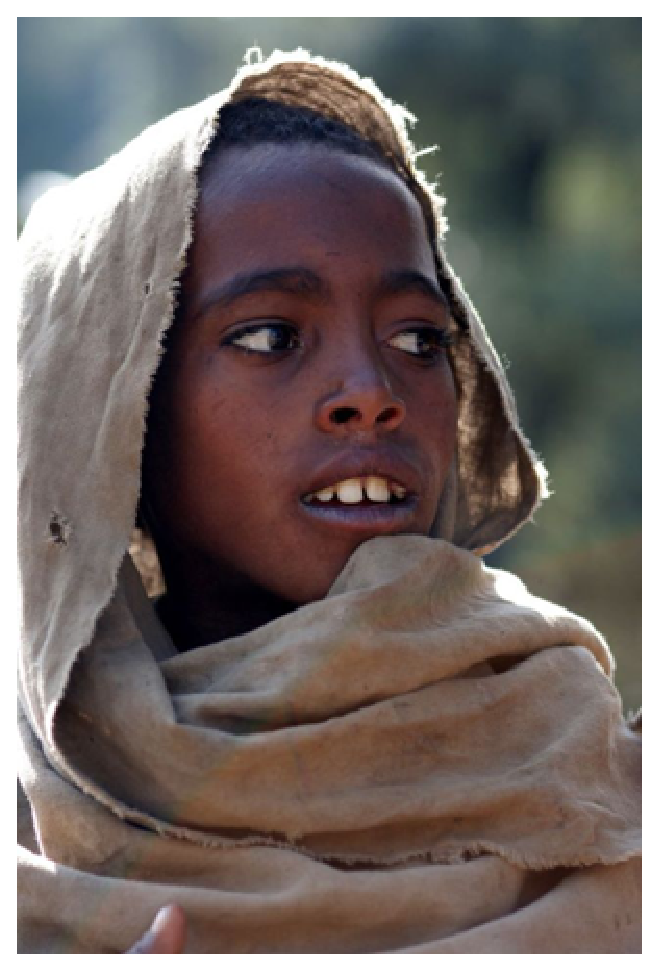
\includegraphics{etiopan.eps}}
    \hspace{-1.5mm}
  \scalebox{-0.43}[0.43]{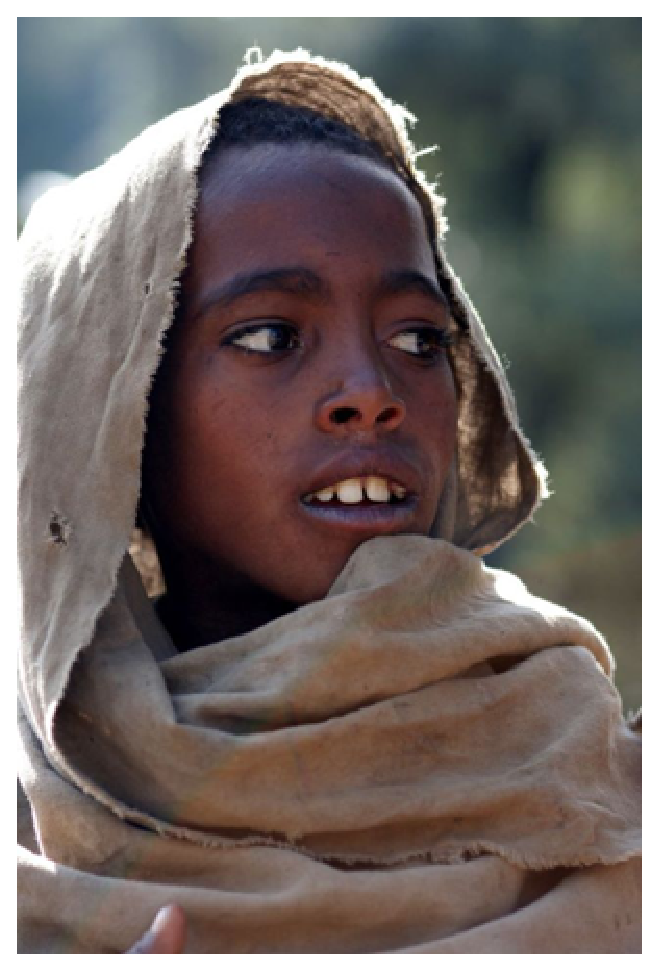
\includegraphics{etiopan.eps}}
  \caption{Malý Etiopánek a jeho bratříček}
  \label{ob_1}
\end{figure*}

\vspace{0.25cm}

\pagebreak

\hspace{-0.5cm} Rozdíl mezi vektorovým \dots

\begin{figure*}[h]
  \centering
  \scalebox{0.43}{
\includegraphics{oniisan.eps}}
  \caption{Vektorový obrázek}
  \label{ob_2}
\end{figure*}

\vspace{0.25cm}

\hspace{-0.5cm} \dots a bitmapovým obázkem

\begin{figure*}[h]
  \centering
  \scalebox{0.7}{
\includegraphics{oniisan2.eps}}
  \caption{Bitmapový obrázek}
  \label{ob_3}
\end{figure*}
\hspace{-0.5cm}se projeví například při zvětšení.

Odkazy (nejen ty) na obrázky \ref{ob_1}, \ref{ob_2} a \ref{ob_3}, na tabulky \ref{tab_1} a \ref{tab_2} a také na algoritmus \ref{Alg_1} jsou udělány pomocí~křížových odkazů. Pak je ovšem potřeba zdrojový soubor přeložit dvakrát.

Vektorové obrázky lze vytvořit i přímo v \LaTeX u, například pomocí prostředí \ \texttt{picture.}

\pagebreak

\begin{landscape}
\begin{figure}[ht]
\begin{picture}(620,360)(0,0)

\put(610,10){\line(0,1){300}}
\put(110,10){\line(0,1){300}}
\put(110,10){\line(1,0){500}}
\put(110,310){\line(1,0){500}}

\put(550,260){\circle{300}}

\put(150,30){\line(0,1){120}}
\put(150,30){\line(1,0){350}}
\put(250,30){\line(0,1){120}}
\put(150,150){\line(1,0){100}}
\put(150,150){\line(2,3){50}}
\put(250,150){\line(-2,3){50}}

\put(160,120){\line(1,0){20}}
\put(160,100){\line(0,1){20}}
\put(160,100){\line(1,0){20}}
\put(180,100){\line(0,1){20}}

\put(160,110){\line(1,0){20}}
\put(170,100){\line(0,1){20}}

\put(220,120){\line(1,0){20}}
\put(240,100){\line(0,1){20}}
\put(220,100){\line(1,0){20}}
\put(220,100){\line(0,1){20}}

\put(220,110){\line(1,0){20}}
\put(230,100){\line(0,1){20}}

\put(160,70){\line(1,0){20}}
\put(160,50){\line(0,1){20}}
\put(160,50){\line(1,0){20}}
\put(180,50){\line(0,1){20}}

\put(160,60){\line(1,0){20}}
\put(170,50){\line(0,1){20}}

\put(220,30){\line(0,1){40}}
\put(240,30){\line(0,1){40}}
\put(220,70){\line(1,0){20}}

\put(230,50){\line(1,0){5}}
\put(235,45){\line(0,1){5}}


\put(250,50){\line(1,0){250}}
\put(250,40){\line(1,0){250}}

\linethickness{1.5pt} 

\put(500,30){\line(0,1){30}}
\put(490,30){\line(0,1){30}}
\put(480,30){\line(0,1){30}}
\put(470,30){\line(0,1){30}}
\put(460,30){\line(0,1){30}}
\put(450,30){\line(0,1){30}}
\put(440,30){\line(0,1){30}}
\put(430,30){\line(0,1){30}}
\put(420,30){\line(0,1){30}}
\put(410,30){\line(0,1){30}}
\put(400,30){\line(0,1){30}}
\put(390,30){\line(0,1){30}}
\put(380,30){\line(0,1){30}}
\put(370,30){\line(0,1){30}}
\put(360,30){\line(0,1){30}}
\put(350,30){\line(0,1){30}}
\put(340,30){\line(0,1){30}}
\put(330,30){\line(0,1){30}}
\put(320,30){\line(0,1){30}}
\put(310,30){\line(0,1){30}}
\put(300,30){\line(0,1){30}}
\put(290,30){\line(0,1){30}}
\put(280,30){\line(0,1){30}}
\put(270,30){\line(0,1){30}}
\put(260,30){\line(0,1){30}}

\linethickness{1pt} 

\put(305,30){\line(0,1){120}}
\put(305,150){\line(-1,-2){20}}
\put(305,130){\line(-1,-2){20}}
\put(305,110){\line(-1,-2){20}}
\put(305,90){\line(-1,-2){20}}
\put(305,150){\line(1,-2){20}}
\put(305,130){\line(1,-2){20}}
\put(305,110){\line(1,-2){20}}
\put(305,90){\line(1,-2){20}}

\put(445,30){\line(0,1){100}}
\put(445,130){\line(-1,-2){20}}
\put(445,110){\line(-1,-2){20}}
\put(445,90){\line(-1,-2){20}}
\put(445,130){\line(1,-2){20}}
\put(445,110){\line(1,-2){20}}
\put(445,90){\line(1,-2){20}}

\put(375,30){\line(0,1){160}}
\put(375,190){\line(-1,-2){20}}
\put(375,170){\line(-1,-2){20}}
\put(375,150){\line(-1,-2){20}}
\put(375,130){\line(-1,-2){20}}
\put(375,110){\line(-1,-2){20}}
\put(375,90){\line(-1,-2){20}}
\put(375,190){\line(1,-2){20}}
\put(375,170){\line(1,-2){20}}
\put(375,150){\line(1,-2){20}}
\put(375,130){\line(1,-2){20}}
\put(375,110){\line(1,-2){20}}
\put(375,90){\line(1,-2){20}}

\end{picture}
\caption{Vektorový obrázek moderního bydlení vhodného pro 21. století. (Buďto vytvořte stejný obrázek, nebo nakreslete pomocí \texttt{picture} váš vlastní domov.)}
\end{figure}
\end{landscape}

\end{document}